\documentclass[10pt,a4paper]{article}
\usepackage[utf8]{inputenc}
\usepackage{amsmath}
\usepackage{amsfonts}
\usepackage[nottoc]{tocbibind}
\usepackage{graphicx}
\usepackage{amssymb}
\usepackage{hyperref}
\author{Stanley}
\title{The Guard Problem}
\newtheorem{theorem}{Theorem}[section]
\newtheorem{corollary}{Corollary}[theorem]
\newtheorem{lemma}[theorem]{Lemma}
\newtheorem{claim}[theorem]{Claim}
\newtheorem{defn}[theorem]{definition}
\newtheorem{proof}[theorem]{proof}

\begin{document}
\maketitle
\tableofcontents
\newpage

\section{Introduction}
\quad In this project, we shall explore the guard problem, first presented by Chvatal in 1975\cite{ref1}, which aims to find the smallest number of guards required to cover a shaped polygon of $n$ verices. Chvatal found that it is occasionally necessary and sometimes sufficient to have $\frac{n}{3}$ guards to cover an $n$-vertex polygon. 

\quad As stated in the problem, we need the minimum number of guards to secure Brian's plot that is shaped as a 24-sided polygon so that he can be assured that its well protected. We consider Brian's farm to be a non-convex polygon, We shall use the theorems of triangulation and colouration to determine the minimum number of guards requuired by Brian. For non-convex polygons, $\frac{n}{3}$ is occasionally necessary and sometimes a sufficient approximation for the minimum number of guards required, whereas for convex polygons we found that a single guards is sometimes sufficient.
\newpage


\section{Simple Polygons}
\paragraph{}
A simple polygon is a polygon  whose line segment do not intersect  itself and it must have no hole. Both convex and non-convex polygons are regarded as simple polygons.

\subsection{One guard Required}
We shall look at some cases of simple polygons where one guard is sufficient to secure the entire perimetre of the polygon.



\begin{figure}[h!]\label{1guard}
\centering
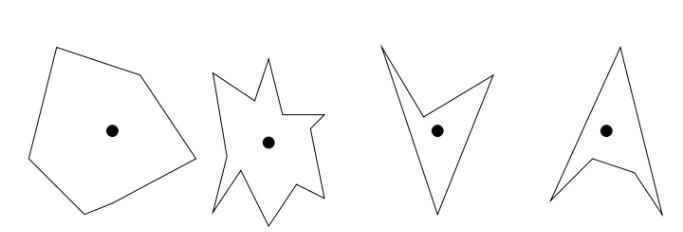
\includegraphics[scale=0.5]{1.jpg}
\caption{Simple polygons where 1 guard is required}
\end{figure}

\subsection{Two guards Required}
Considering a 6-sided non-convex polygon, two guards are required to secure the interior of the polygon.

\begin{figure}[h!]\label{2guard}
\centering
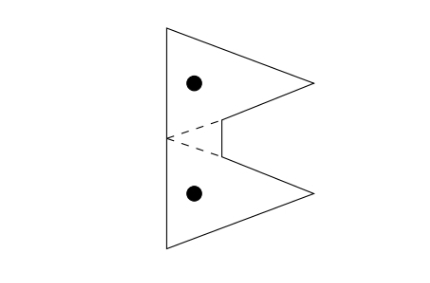
\includegraphics[scale=0.5]{2.jpg}
\caption{Simple polygons where 2 guard is required}
\end{figure}
\paragraph{•}
Now we want to generalize and determine the number of guards for any n-sided simple polygon, to do this we shall introduce the Triangulation and Colouration theorems.

\begin{theorem}
Every simple polygon has a triangulation
\end{theorem}
We shall prove that every simple polygon can indeed be triangulated, we shall prove this by induction.
\begin{figure}[h!]\label{triangle}
\centering
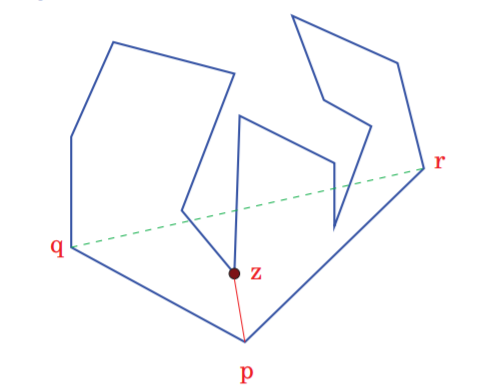
\includegraphics[scale=0.2]{3.png}
\caption{Triagulation}
\end{figure}
\\
\begin*{proof:}
Considering the very trivial case of a polygon P where $n=3$, P is infact triangulated. Considering the figure above \ref{1guard}, Pick a convex vertex $p$. Let $q$ and $r$ be neigbouring vertices, if $qr$ a diagonal, add it, By Induction, the smaller plygon has a triangulation. If $qr$ not a diagonal, let $z$ be the reflex vertex farthest to $qr$ inside $\bigtriangleup pqr$, add additional $pz$; subpolygons on both sides have a triangulation.
\end{proof}


\begin{theorem}
Every triangulation of a polygon P with n vertices has $n-2$ triangles and $n-3$ diagonals
\end{theorem}
\\
\begin*{Proof:}	
We prove this by induction, considering the trivial case of $n=3$, the statement is trivially true. Next we assume it is true for all $n$ polygons. Next we pick a diagonal $d$ joining the vertices $q$ and $r$, cutting the polygon P into two $P_{1}$ and $P_{2}$, having  $n_{1}$ and  $n_{2}$ vertices respectively,since $q$ and $r$ appear in both sub-polygons, we know that $n_{1} + n_{2}=n +2$. 
The induction hypothesis assumes that there are $\left( n_{1}-2\right) + \left( n_{2} -2\right)$ in $P_{1}$ and $P_{2}$ respectively. Hence $P$ has\\
$$\left( n_{1}-2\right) + \left( n_{2} -2\right)= \left(n_{1} + n_{2}\right)-4= \left(n+2\right)-4=\left( n-2\right)$$\\
$\left( n-2\right)$triangles. Similarly, $P$ has $\left( n_{1}-3\right)+\left( n_{2}-3\right)+1=n-3$ diagonals
\end{proof}


\begin{theorem}
The polygon produced upon triangulation is 3 colourable
\end{theorem}
\\
\begin{Proof}
For the trivial case where n=3, this holds true because we can assign three colours to all three vertices. Suppose we have a larger polygon with vertex $n$, now we can assign colours to this polygon  starting from the edge, the first two colours are assigned to first two edges and then the third verted would have the third colour. These three colours form the pattern within which other triangles in the polygon are coloured such that each triangle is composed of these distinct colours.
\end{Proof}


\begin{figure}[h!]\label{colouration}
\centering
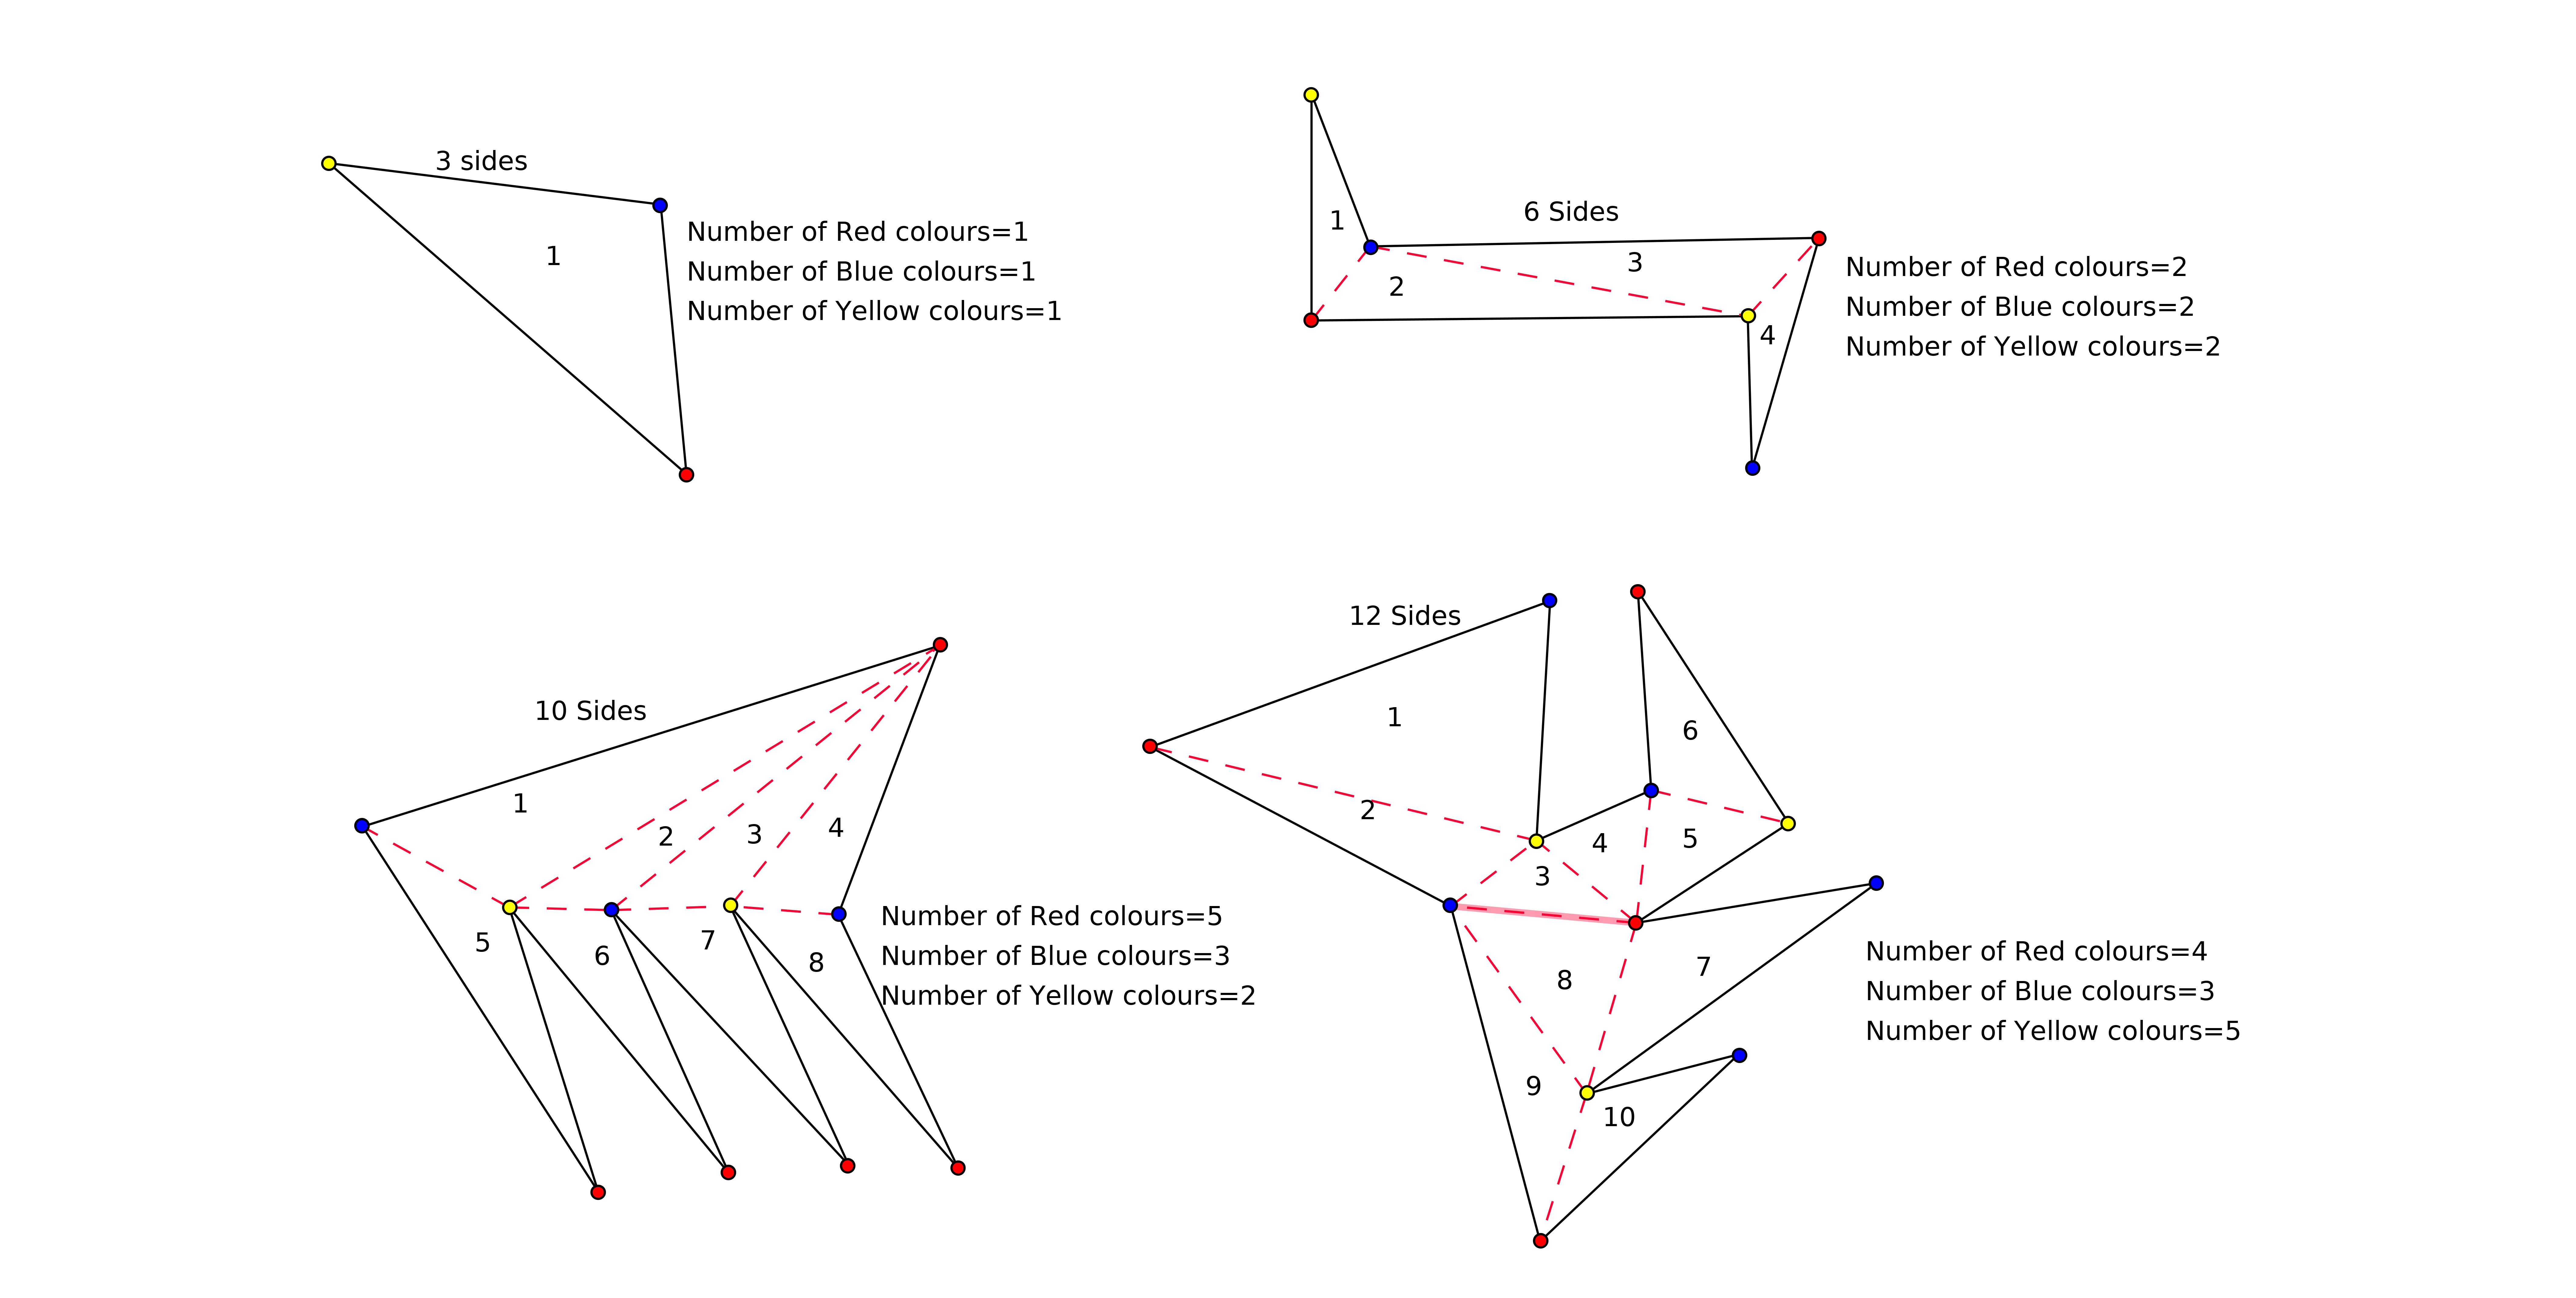
\includegraphics[width=12.0cm,height= 15.5cm]{image1.png}
\caption{Triangulated and Coloured polygons}
\end{figure}
\newpage
\section{MInimum number of guards determination}

We shall apply the aforementioned theorems to determine the minimum number of guards for any $n$-vertex polygon, this is achieved by calculating the number of times the various colours appear in the diagram, the minimum number of guards will be equal to the number colour of that appears least, therefore the guards must be placed at the points where the minimum colour appears.
\newpage
\begin{figure}[h!]\label{colouration}
\centering
\includegraphics[width=12.0cm,height= 15.5cm]{image2.png}
\caption{Minimum Guards}
\end{figure}

Looking at the 17-sided polygon above, the minimum number of guards corresponds to the colour that appears least on the diagram, since both red and blue colours appaers least(i.e 5 times each), the minimum number of guards must be placed at these positions, similarly, the minimum number of guards for the 18-sided polygon will either be on the red or yellow colour since they both appear 5 times each 


\subsection{Brians 24-sided polygon farm}
We shall use the same principles discussed above to determine the minimum number of guards for brian's farm, the figure below shows the triangulated and colured structure of Brian's farm.
\begin{figure}[h!]\label{colouration}
\centering
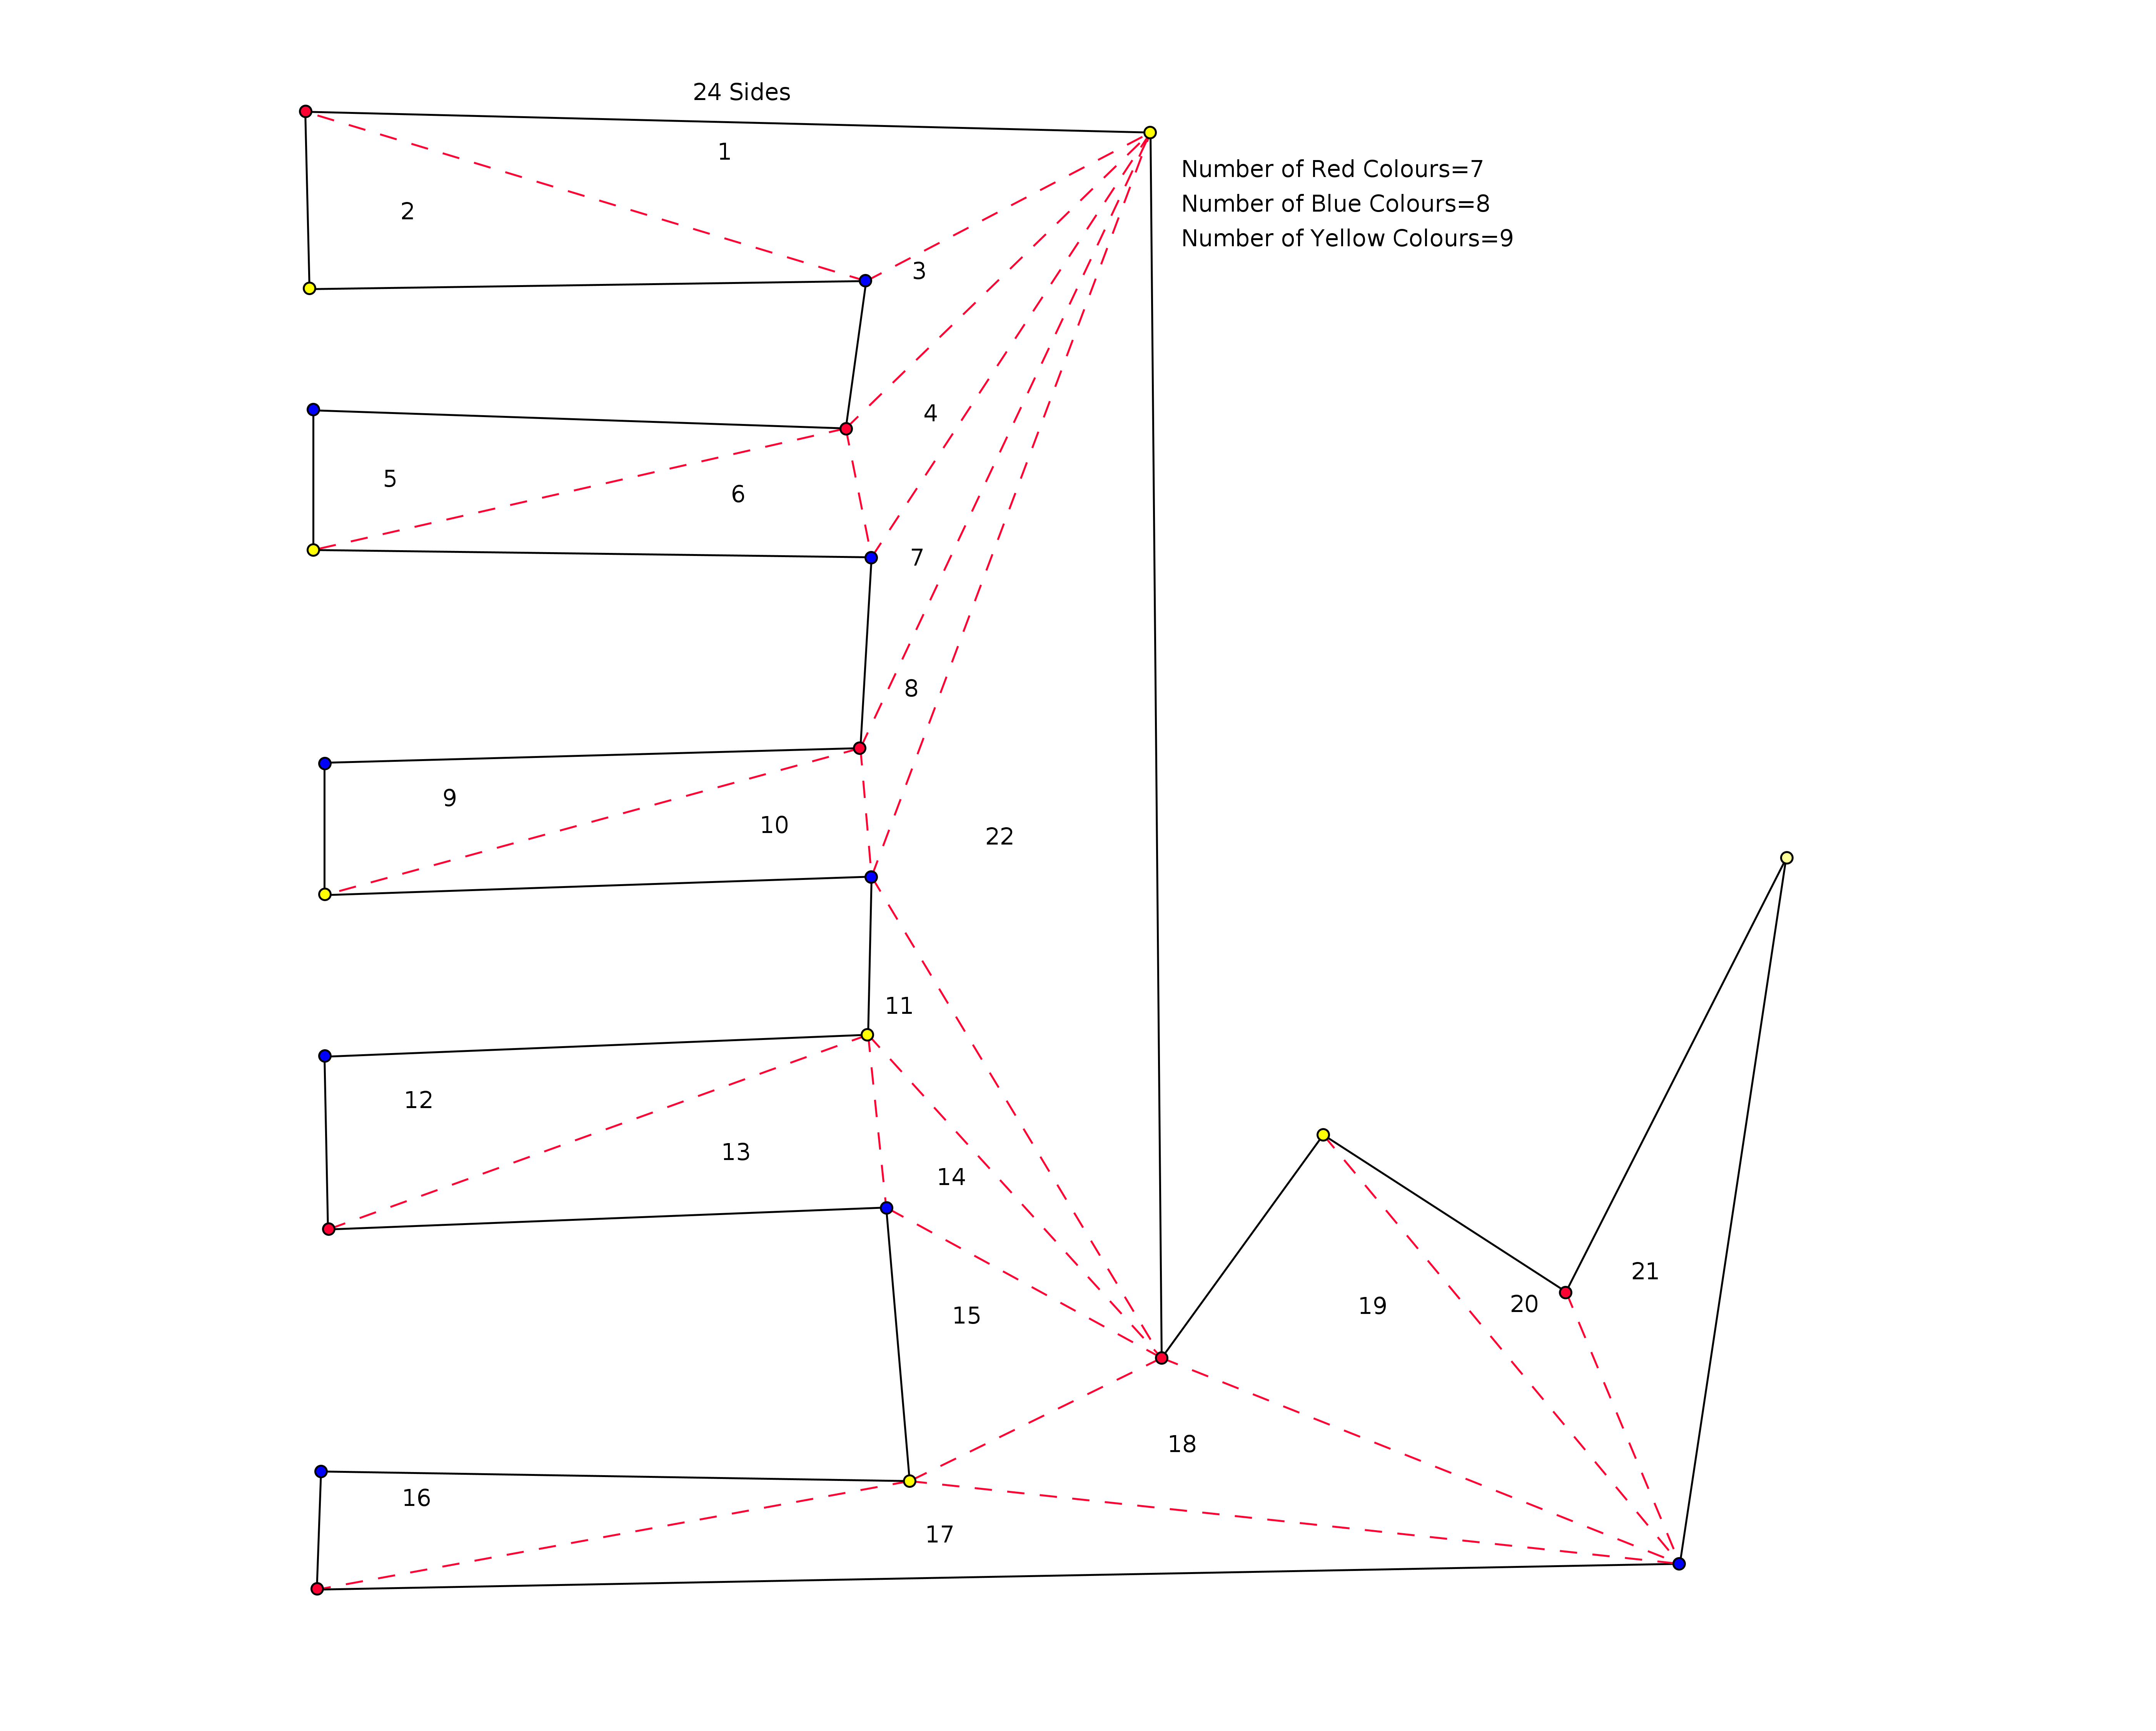
\includegraphics[width=12.0cm,height= 15.5cm]{image3.png}
\caption{Brian's Farm}
\end{figure}
\\
The minimum number of guards required by Brian to secure the entire perimetre of his farm is 7, this is given by the number of red colours on the diagram. 
\newpage
\section{Conclusion}
The minimum number of guards required by Brian to secure the entire perimeter of his farm is 7 as indicated by the red colours of the 24-sided polygons. 

The number of guards required to cover any n-gon shaped field is proportional to the number of sides of the polygon, the solution is found by taking the floor of $\frac{n}{3}$ where $n$ is the number of sides of the n-gon, however this value is not often the minimum number of guards required.

\bibliographystyle{unsrt}
\bibliography{maths.bib}

\end{document}